\section{\Large PROBLEM SET 7}
\subsection{PROBLEM 1}
\textit{Introduce representative (from manufacturer or Wertz or first lectures) sensor errors in the form of constant bias and Gaussian noise with given standard deviation.}

As the specific data regarding for NISAR ADCS sensors are not widely available, much of the sensor error and bias information was extrapolated from data from Wertz and lecture materials, as well as manufacturers of sensors for similar satellites. The table below includes the general sensor information used in this analysis.

\begin{table}[H]
\centering
\begin{tabular}{|l|l|l|}
\hline
\textbf{Sensor} & \textbf{Sensor Error} & \textbf{Sensor Bias} \\ \hline
Sun Sensor \cite{Wertz} & 0.5\degree & 0\degree \\ \hline
Star Tracker \cite{Wertz} & 0.01\degree & 0\degree \\ \hline
Gyroscope \cite{CVGGyro} & 0.001\degree / s & 5E-5\degree/s \\ \hline
\end{tabular}
\end{table}

\subsection{PROBLEM 2}
\textit{Re-apply the attitude determination algorithms from the previous pset. Plot attitude estimation error. Note that the attitude estimation error represents a rotation matrix (DCM) which quantifies how far the estimated attitude is from the true attitude. You can use any parameterization to plot the attitude estimation errors corresponding to this DCM. Is the result consistent with the sensor bias and noise you have introduced?}

The estimation errors for the deterministic method, q-method, and kinematics-based method are plotted below. As expected, the q-method has a significantly lower error than the deterministic method. Additionally, since the gyroscopes were modeled to have a slight bias, the Euler angles slowly drift away from expected values.

\begin{figure}[H]
\centering
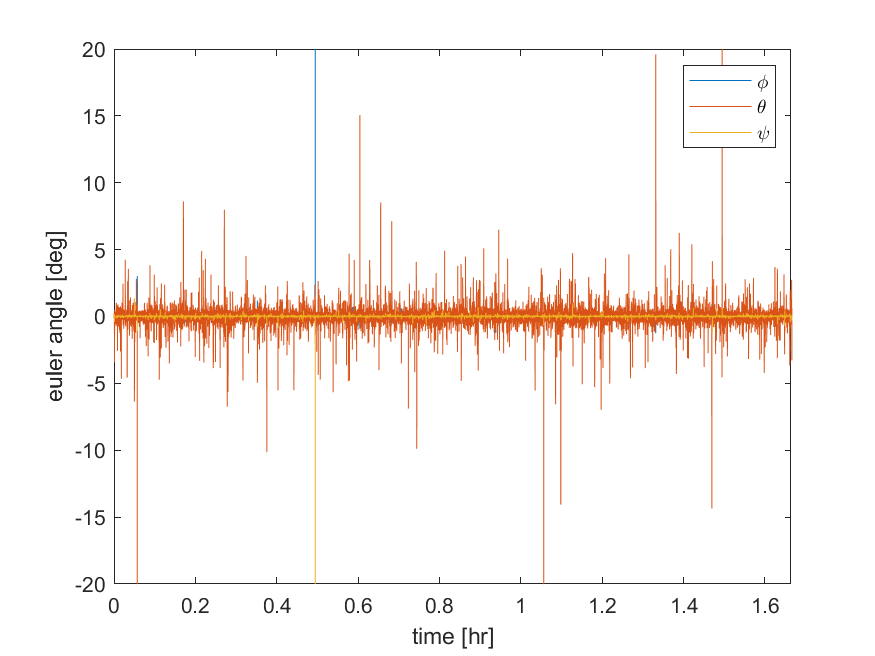
\includegraphics[scale=0.6]{Images/ps7_problem2_DADFict.png}
\caption{Attitude error using deterministic attitude determination}
\label{fig:ps7_problem2_DADFict}
\end{figure}

\begin{figure}[H]
\centering
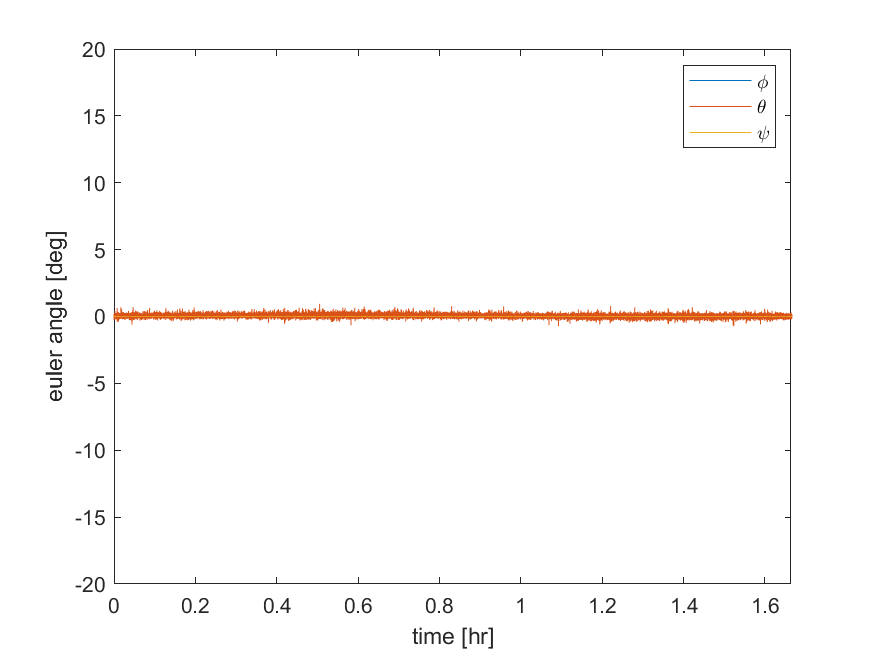
\includegraphics[scale=0.6]{Images/ps7_problem2_qMethod.png}
\caption{Attitude error using q-method}
\label{fig:ps7_problem2_qMethod}
\end{figure}

\begin{figure}[H]
\centering
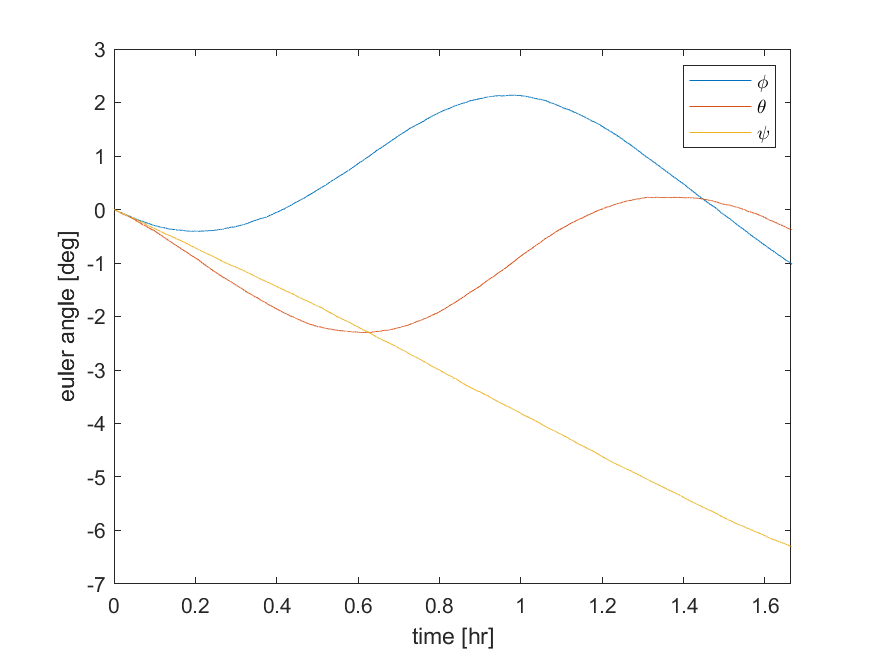
\includegraphics[scale=0.6]{Images/ps7_problem2_kin.png}
\caption{Attitude error using kinematic attitude determination}
\label{fig:ps7_problem2_kin}
\end{figure}

\subsection{PROBLEM 3}
\textit{For small sensor errors, the DCM corresponds to a small rotation. Can you give an interpretation of small angles (e.g., in Euler angles and quaternions) to the obtained error DCM?}

For this analysis, we choose to use q-method, as it produced the smallest errors in the previous section. In order to estimate the size of the errors, we compare the exact error DCM to the small angle approximation DCM based on the corresponding Euler angles, shown below.
\begin{align*}
    A_{\text{small angle}} &= 
    \begin{bmatrix}
        1 & \phi & -\psi \\
        -\phi & 1 & \theta \\
        \psi & -\theta & 1
    \end{bmatrix}
\end{align*}

The Frobenius norm is then calculated from the difference in the error DCM and small angle DCM to see how applicable small angle assumptions are for the error. Based on Figure \ref{fig:ps7_problem3}, the magnitudes of the Frobenius norm reflect that the overall errors were relatively small for the q-method, implying only a very small angular difference.

\begin{figure}[H]
\centering
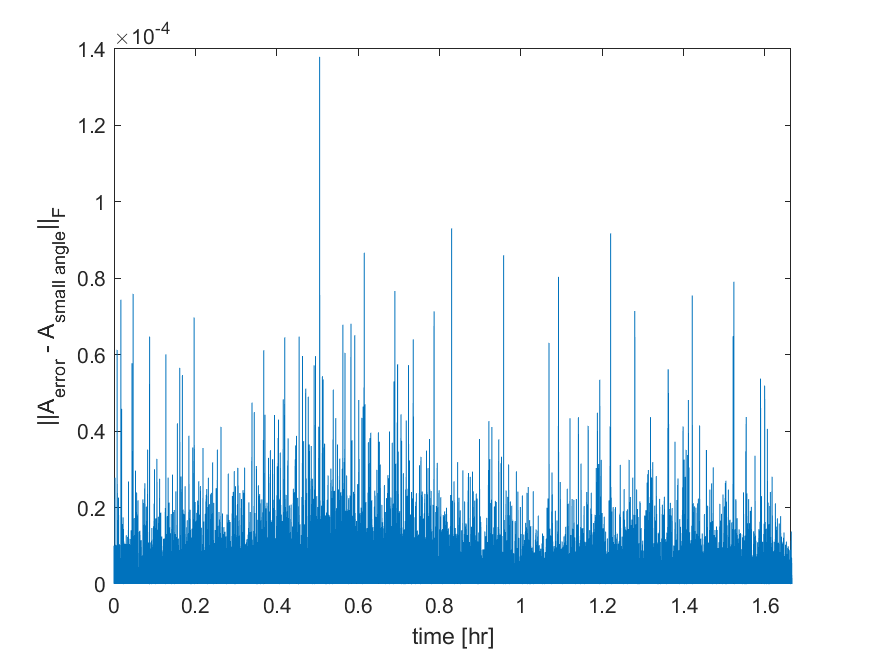
\includegraphics[scale=0.6]{Images/ps7_problem3.png}
\caption{Frobenius norm of error estimate versus small angle approximation}
\label{fig:ps7_problem3}
\end{figure}

\subsection{PROBLEM 4}
\textit{Start modeling actual sensors in dedicated (Simulink or otherwise) subsystems which are part of the spacecraft. These models take inputs from ground-truth simulation and provides output measurements, including systematic and random errors. Take inspiration from overview of sensors discussed in class and textbook for typical errors.}

There are three major types of sensors used in this analysis: sun sensors, star sensors, and gyroscopes. The following section discusses the basics of each sensor's function and modeling.

Sun sensors utilize a photoelectric effect to produce an electric current based on the Sun's emitted electromagnetic radiation. For a single sensor, the current is based on sensitive surface $S$, optical properties $\alpha$, and angle of incidence $\theta$.
\begin{align*}
    I = \alpha S \cos(\theta)
\end{align*}

Due to the nonlinearity of this relationship, sun sensors operate within a limited field of view where the relationship between the angle of incidence and current draw is approximately linear.

However, because NISAR operates in a sun-synchronous orbit, the sun sensor model we used did not factor in the sensor's field of view, as a well-placed sensor with a wide enough FOV will always have the sun in frame. Our sun sensor model outputs the direction of the Sun from the simulation and adds Gaussian noise.

Star trackers are more complicated. These sensors are similar to cameras that capture star positions and compare them to an existing star catalog, which can be used to determine the satellite's attitude. These trackers are often designed to have a much narrower field of view to maximize the pixel pitch. Star trackers use algorithms such as angular separation matching to match each star to a star in the star catalog.

The star tracker model used in our simulations introduces simplifying assumptions. The model we use generates 10 random unit vectors within the FOV of the star tracker on board (approximately $20 \degree$) and adds Gaussian noise. These random vectors represent the direction of 10 arbitrary stars in the celestial sphere.

Gyroscopes measure the angular velocity of the satellite. There are two main types of gyroscopes: laser gyroscopes and mechanical gyroscopes. Laser gyroscopes emit light along a fiber optic cable ring in opposite directions. The time or phase difference of the light along the ring can be used to compute the angular velocity. Mechanical gyroscopes, such as rate gyros, use gimbals and measure the angle induced in one direction by angular velocity in another. This measurement can come from a device such as a potentiometer, which provides an electrical voltage signal.

To simplify the model of the sensor, the gyroscope model takes angular velocity from the simulation and adds Gaussian noise and expected bias.

\begin{figure}[H]
\centering
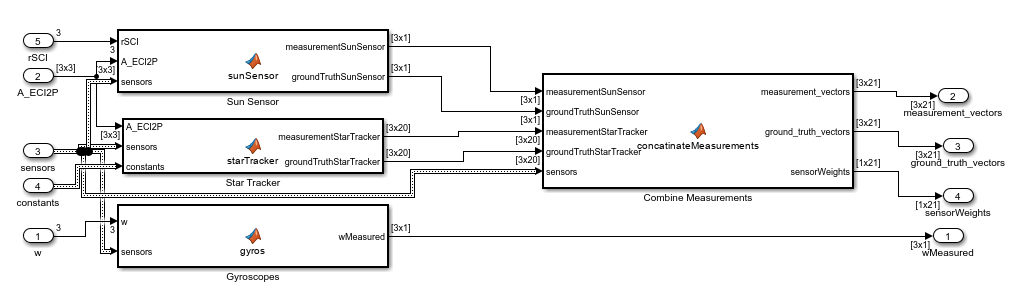
\includegraphics[scale=0.59]{Images/ps7_problem4_simulink.png}
\caption{Simulink model of sensors}
\label{fig:ps7_problem4_simulink}
\end{figure}

\begin{figure}[H]
\centering
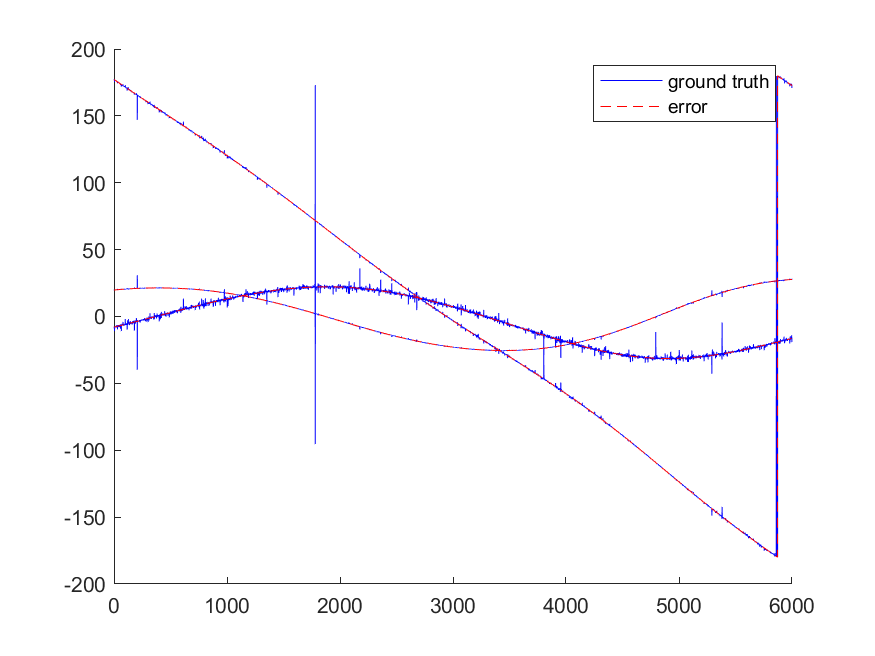
\includegraphics[scale=0.6]{Images/ps7_problem4_DADFict.png}
\caption{Attitude error using deterministic attitude determination}
\label{fig:ps7_problem4_DADFict}
\end{figure}

\begin{figure}[H]
\centering
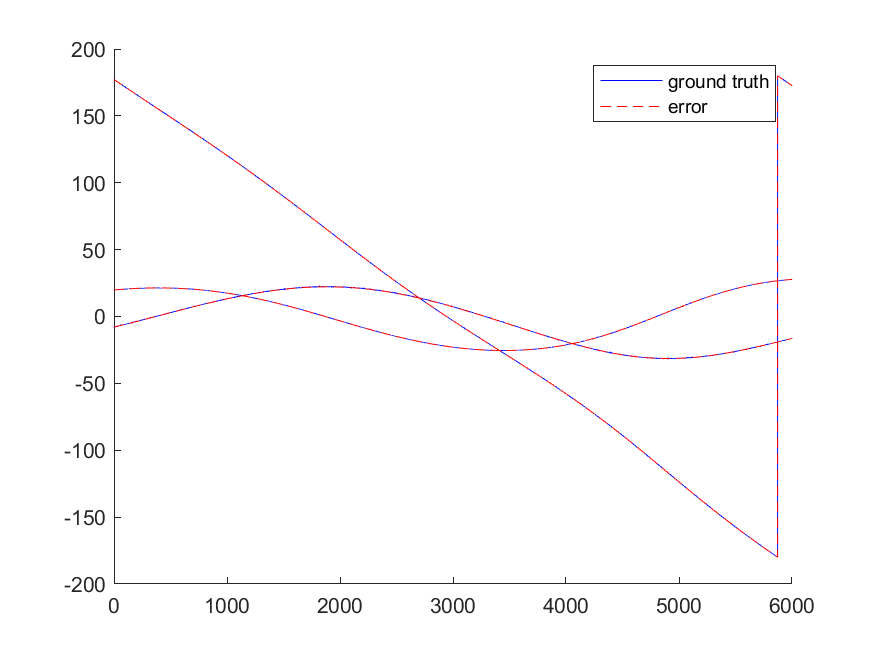
\includegraphics[scale=0.6]{Images/ps7_problem4_qMethod.png}
\caption{Attitude error using q-method}
\label{fig:ps7_problem4_qMethod}
\end{figure}

\begin{figure}[H]
\centering
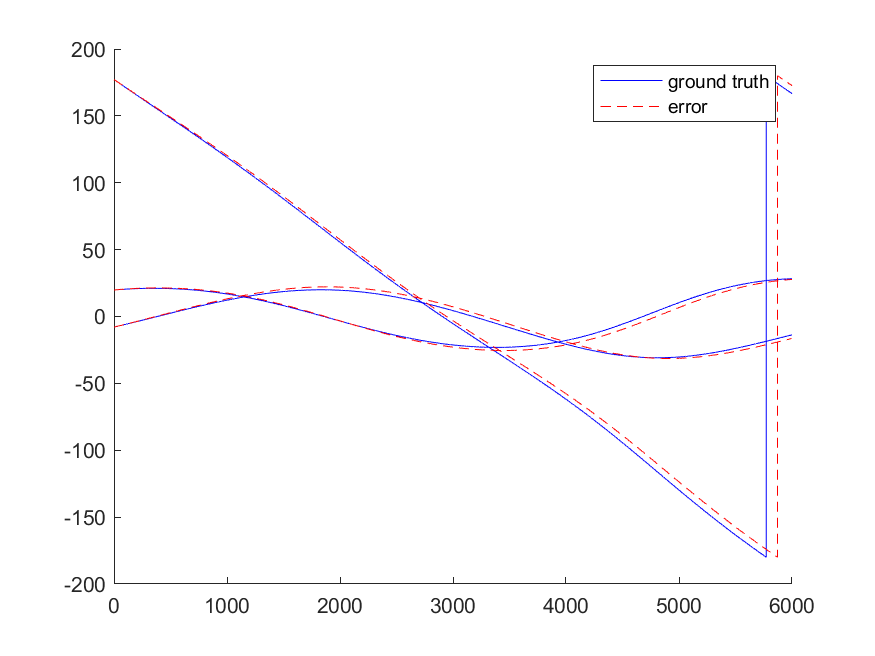
\includegraphics[scale=0.6]{Images/ps7_problem4_kin.png}
\caption{Attitude error using kinematic attitude determination}
\label{fig:ps7_problem4_kin}
\end{figure}

\subsection{PROBLEM 5}
\textit{Designing and implement the time update of a KF/EKF to obtain the best estimate of the state from the available measurements and models:}

The following MATLAB function is our time update-only implementation of a multiplicative extended Kalman filter (MEKF). We describe the formulation of the MEKF immediately following this function.

\lstinputlisting{src/timeUpdate.m}

\textit{Search in literature, define, and code a state transition matrix $\Phi$ which provides your state at step k+1 based on the state at step k. Verify that the output of this propagation step is consistent with the rigorous propagation of the attitude (numerical integration). Plot propagation errors as needed.}

Our state consists of 3 small angles (zero mean) and angular velocities. Our state does not track the attitude directly, but we can compute quaternions using known kinematics.
\begin{align*}
    \Vec{x} = \begin{bmatrix}
        \alpha_{x} & \alpha_{y} & \alpha_{z} & \omega_{x} & \omega_{y} & \omega{z}
    \end{bmatrix}^{\intercal}
\end{align*}

The small angle component of our state is reset every iteration and not updated in the time update step \cite{CubeSatTelescope}.
\begin{align*}
    A &= I_{3} + \frac{s_{\omega}}{\omega} [\Vec{\omega}_{t} \times] + \frac{1 - c_{\omega}}{\omega^{2}} [\Vec{\omega}_{t} \times] [\Vec{\omega}_{t} \times] \\
    \Phi_{\omega} & = I_{3} + \Delta t \begin{bmatrix}
        0 & \frac{I_{y} - I_{z}}{I_x} \omega_{z_{t}} & \frac{I_{y} - I_{z}}{I_x} \omega_{y_{t}} \\
        \frac{I_{z} - I_{x}}{I_y} \omega_{z_{t}} & 0 & \frac{I_{z} - I_{x}}{I_y} \omega_{x_{t}} \\
        \frac{I_{x} - I_{y}}{I_z} \omega_{y_{t}} & \frac{I_{x} - I_{y}}{I_z} \omega_{x_{t}} & 0
    \end{bmatrix} \\
    \Phi &= \begin{bmatrix}
        A & 0 \\
        0 & \Phi_{\omega}
    \end{bmatrix}
\end{align*}

Since we are using a MEKF, we propagate the quaternion attitude representation outside of the state vector. The quaternion attitude is propagated by $\Omega (\Vec{\omega})$, identical to the quaternion kinematics used previously.

We plot the attitude from our MEKF and our numerical integration simulation, respectively. Upon inspection, these plots appear identical. Small errors in the simulation are analyzed later in Problem 6.

\begin{figure}[H]
\centering
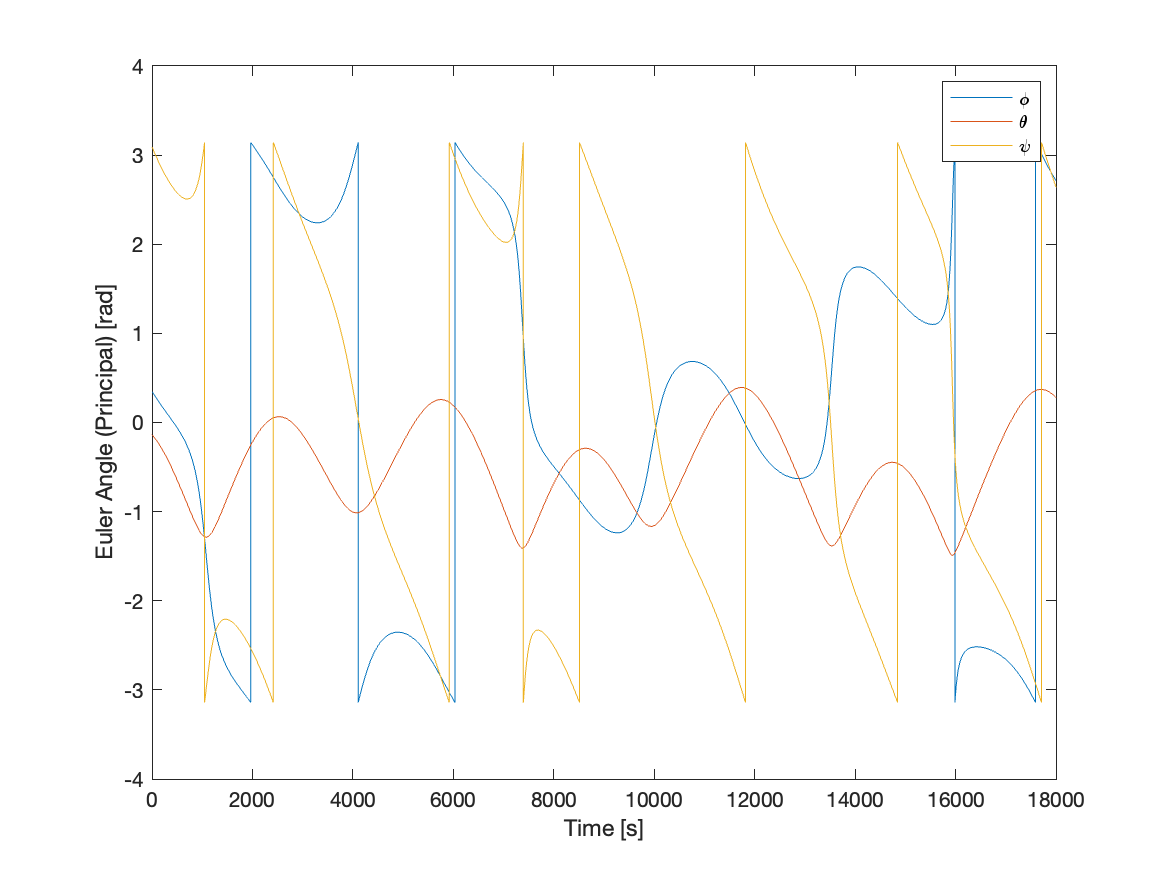
\includegraphics[scale=0.6]{Images/ps7_problem5a_angle_est.png}
\caption{Attitude evolution based on MEKF time update}
\label{fig:ps7_problem5a_angle_est}
\end{figure}

\begin{figure}[H]
\centering
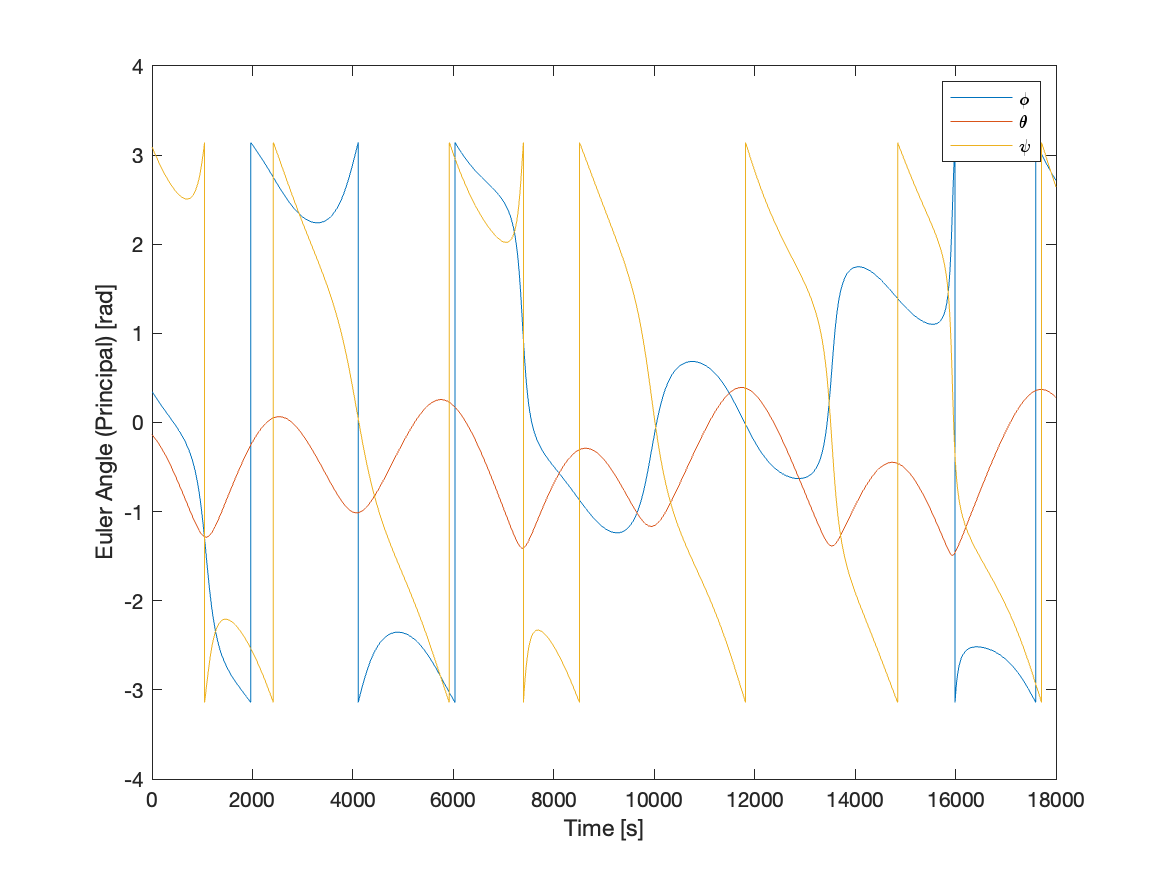
\includegraphics[scale=0.6]{Images/ps7_problem5a_angle_sim.png}
\caption{Attitude evolution from "ground truth" simulation}
\label{fig:ps7_problem5a_angle_sim}
\end{figure}

We also plot the angular velocity from both the MEKF time update step and the numerical simulation. As with the attitude evolution, both plots appear to be the same. Note that we do not include perturbations in our simulation in our comparison, as the state would quickly diverge otherwise because the measurement update is not yet implemented in the MEKF.

\begin{figure}[H]
\centering
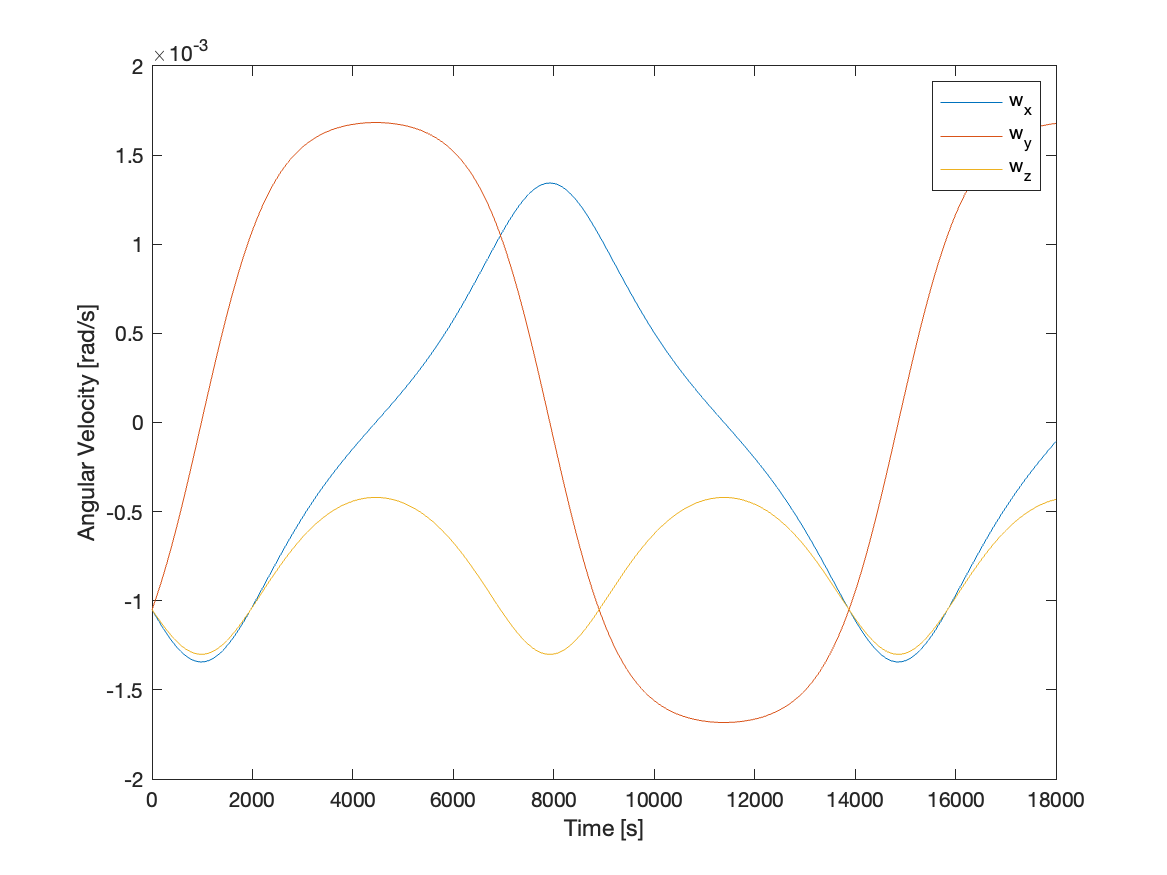
\includegraphics[scale=0.6]{Images/ps7_problem5a_angvel_est.png}
\caption{Angular velocity based on MEKF time update}
\label{fig:ps7_problem5a_angvel_est}
\end{figure}

\begin{figure}[H]
\centering
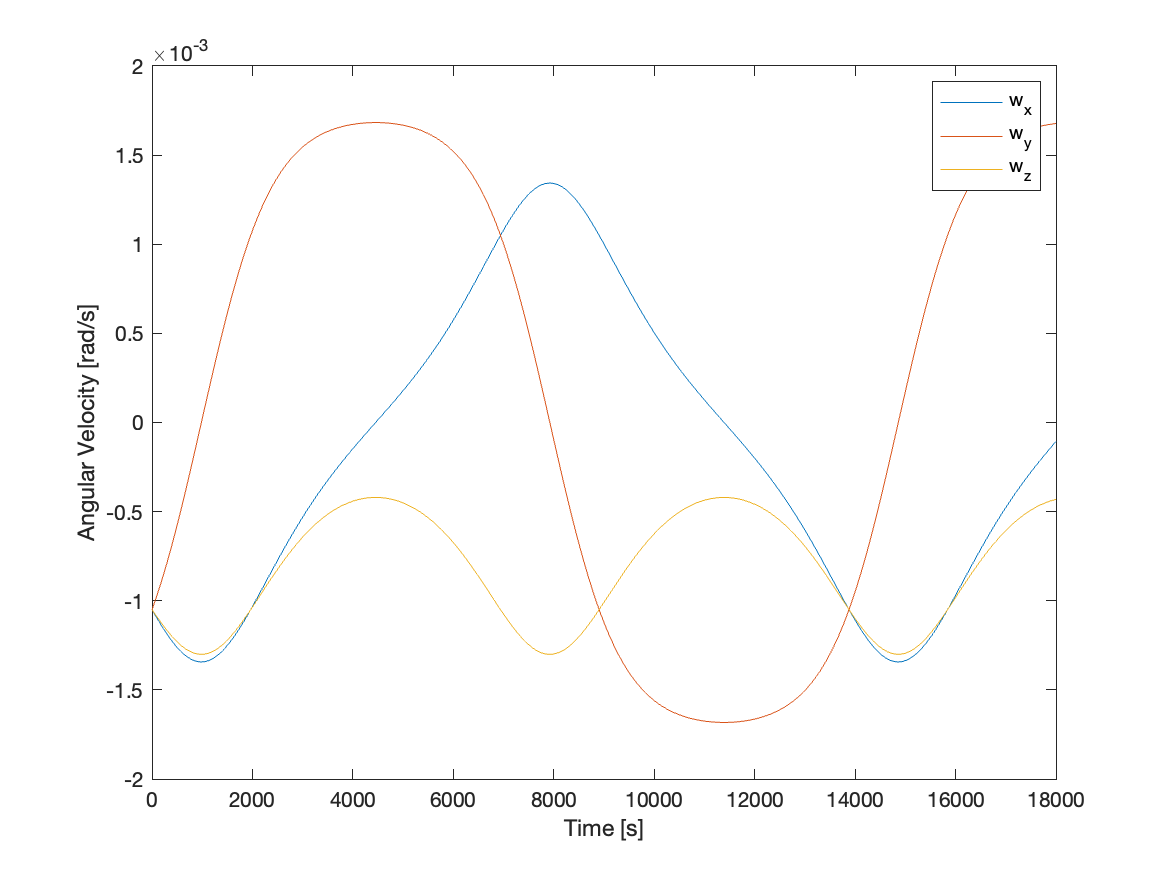
\includegraphics[scale=0.6]{Images/ps7_problem5a_angvel_sim.png}
\caption{Angular velocity from "ground truth" simulation}
\label{fig:ps7_problem5a_angvel_sim}
\end{figure}

\textit{Search in literature, define, and code a control input matrix B which provides the increment to your state at step k+1 due to a control torque at step k. Hint: optional at this stage since you do not have a controller yet.}

For now, we choose to model our control inputs as torque inputs (moments) about the principal axes. Thus, we can choose a $B$ matrix as follows:
\begin{align*}
    u_{t} &= \begin{bmatrix}
        M_{x_{t}} & M_{y_{t}} & M_{z_{t}}
    \end{bmatrix} \\
    B &= \Delta t \begin{bmatrix}
        \frac{1}{I_{x}} & 0 & 0 \\
        0 & \frac{1}{I_{y}} & 0 \\
        0 & 0 & \frac{1}{I_{z}}
    \end{bmatrix}
\end{align*}

\textit{(a) and (b) allow you to propagate the state from k to k+1 including the known control input torques. Hint: Initially you will design the filter by neglecting any control torque from your simulation.}

We have not yet implemented a controller at this step. As such, we will run the MEKF with $u_{t} = 0$ for now.

\textit{Define and code an initial state error covariance matrix P which quantifies the uncertainty of your initial state. This can be picked as diagonal matrix with diagonal elements representing the variance of each state parameter $\sigma^{2}$. Initially you can neglect cross-covariance terms assuming that errors of various state components are not correlated.}

We can choose our initial state error covariance matrix $P$ as a diagonal matrix, with the diagonal entries corresponding to $\alpha$ set to $1$ and the entries corresponding to $\omega$ to the variance computed from angular velocity history. This can be collected as statistics from the propagation shown previously. Once the entire MEKF is implemented, this matrix should converge over time. For now, the state error covariance matrix $P$ has no impact on the output of just our time update.

\textit{The time update of the EKF needs $\Phi$, B, and P. Hint: You could increment your navigation performance by keeping the filter receptive to new measurements at steady state through the addition of constant process noise Q at each step. Initially you can define Q similar to P but much smaller (e.g., 1/10 or 1/100).}

For the purpose of this section, we arbitrarily define $Q = P_{t=0} \times 0.01$.

\subsection{PROBLEM 6}
\textit{Produce plots showing true attitude estimation errors (estimate vs truth with statistics), formal or estimated attitude estimation errors (covariance from filter). Discuss the results, do they meet expectations? How well is the true estimation error described by the formal covariance? Note that we are only implementing the time update even if we call them “attitude estimates and estimation errors”.}

We show plots of errors for the attitude and angular velocity. We can see that the angular velocity error is very low, reaching a maximum of $10^{-7}$ over three orbits. Note that our raw attitude representation is in quaternions, but we convert to Euler angles for visualization. The Euler angle error is somewhat larger, beginning initially around $10^{-7}$ and ending around $10^{-3}$ over the course of the three orbits. The Euler angle error is possibly larger because there is a compounding effect of errors in computing angular velocity.

\begin{figure}[H]
\centering
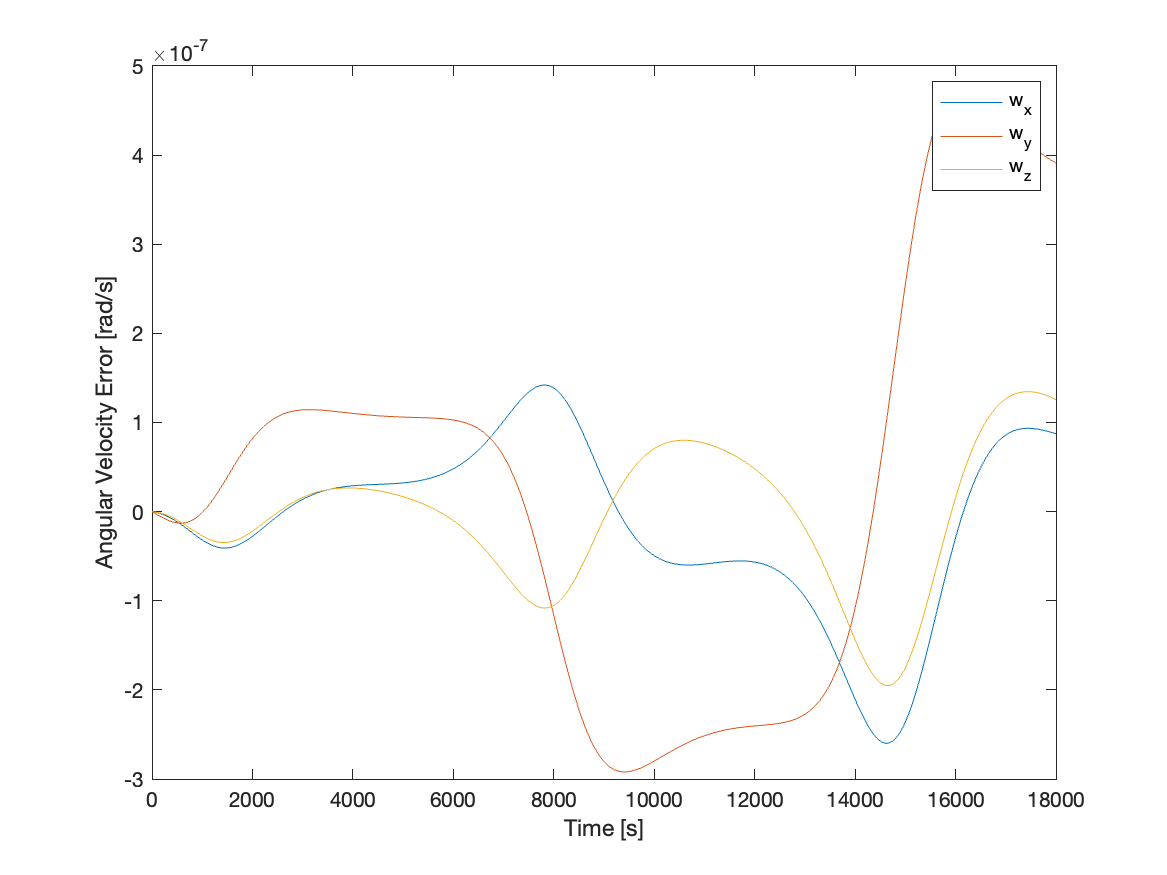
\includegraphics[scale=0.6]{Images/ps7_problem6_angvel_err.png}
\caption{Attitude error between estimate and simulation}
\label{fig:ps7_problem6_angvel_err}
\end{figure}

\begin{figure}[H]
\centering
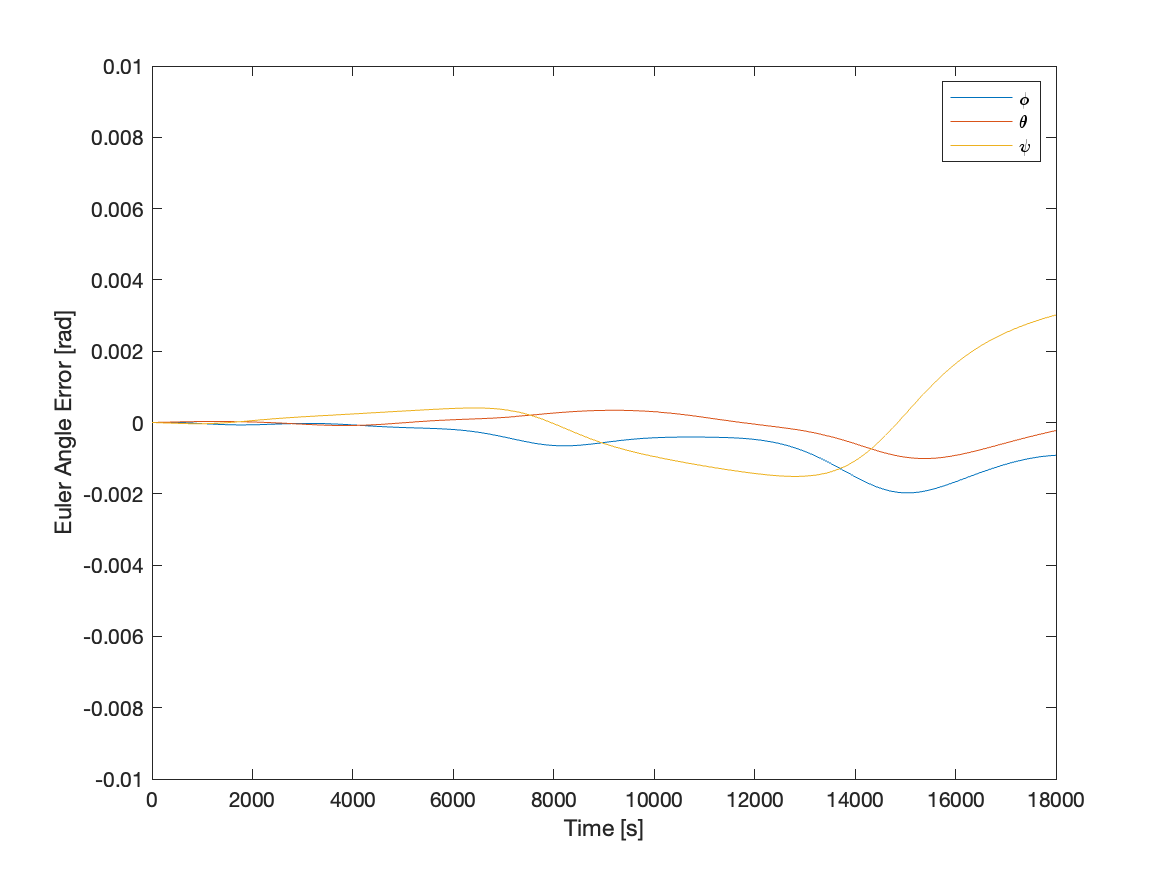
\includegraphics[scale=0.6]{Images/ps7_problem6_angle_err.png}
\caption{Angular velocity error between estimate and simulation}
\label{fig:ps7_problem6_angle_err}
\end{figure}

These results are within expectations, as we do not have a modeled measurement update step that could help reduce our errors. Also, our injected process noise $Q$ is not beneficial to the time update alone, as $Q$ is intended to help accommodate measurement updates.